\documentclass{article}
\usepackage[utf8]{inputenc}
\usepackage{amsmath}
\usepackage{amssymb}
\usepackage{amsfonts}
\usepackage{graphicx}
\usepackage{tikz}
\usetikzlibrary{angles,fit,arrows,calc,math,matrix,intersections,through,backgrounds,cd}
\usepackage{pgfplots}
\pgfplotsset{compat=1.18}
\usepackage{geometry}
\geometry{a4paper, margin=1in}
\usepackage{booktabs} % For professional looking tables

\title{Systematic Study of $K$ Values in Global Arithmetic Torsion for the $4_1$ Knot}
\author{Manus}
\date{\today}

\begin{document}
\maketitle

\section{Introduction}
This document outlines a research direction focused on the systematic study and pattern recognition of the integer $K$ that appears in the global arithmetic torsion formula, $\mathcal{T}(S) = \Delta(t)(t^K-1)$, specifically for the figure-eight knot ($4_1$). This investigation aims to understand the conditions under which $K$ takes certain values, particularly $K=0$, by analyzing various paths (relators) in the knot group $G(4_1)$.

The figure-eight knot, denoted as $4_1$, is a prime, alternating knot with a crossing number of four. It is the simplest hyperbolic knot and plays a significant role in knot theory and related fields due to its rich mathematical structure.

\begin{figure}[h!]
    \centering
    \documentclass{standalone}
\usepackage{amsthm}
\usepackage{amssymb}
\usepackage{amsfonts}
\usepackage{amsmath}
\usepackage{mathtools}

\usepackage{pgf}
\usepgflibrary{fpu}
\usepackage{pgfplots}
\usepackage{tikz}
\usetikzlibrary{angles,fit,arrows,calc,math,matrix,intersections,through,backgrounds,cd}
\usepackage{tkz-euclide}
\usepackage{tkz-graph}
\usepackage{graphicx}
\pgfplotsset{compat=1.18}

\begin{document}

        \tikzmath{
                \one = 1;
                \base = 2.618033988749;
                \offset = 15.8888888;
                \valofpi = 3.1415926;
                \anglei = 3.1415926;
                \angleo = 3.1415926;
        }

        \begin{tikzpicture}[scale=1.0]
                % 1. 绘制坐标轴
                \draw[black, line width=0.6pt, ->]
                (\offset,0) to[out=90,in=270] (\offset,15.5)
                node [anchor=south] {y};

                \draw[black, line width=0.6pt, ->]
                (-7.5,0) to[out=0,in=180] (18,0)
                node [anchor=west] {x};

                % 2. 绘制 x 和 y 坐标轴刻度
                \foreach \x in {-25,...,2} {
                        \node [anchor=north] at (\x/9*8 + \offset, 0) {\x};
                }
                \foreach \y in {1,...,17} {
                        \node [anchor=-135] at (18, \y/9*8) {\y};
                }

                % 3. 浅灰色水平网格线
                \foreach \t in {17,...,1} {
                        \draw [lightgray, line width=0.6pt]
                        (-7.5,\t/9*8)
                        to[out=0,in=180]
                        (18,\t/9*8);
                }

                % 4. 浅灰色竖直网格线
                \foreach \t in {-26,...,2} {
                        \draw [lightgray, line width=0.6pt]
                        (\t/9*8 + \offset, 0)
                        to[out=90,in=270]
                        (\t/9*8 + \offset, 15.5);
                }




        \end{tikzpicture}
\end{document}

    \caption{The Figure-Eight Knot ($4_1$).}
    \label{fig:knot_4_1}
\end{figure}

\section{Background: Global Arithmetic Torsion}
The concept of global arithmetic torsion, as introduced in the provided research materials (Material 5), is given by the expression $\mathcal{T}(S) = \Delta(t)(t^K-1)$. Here, $\Delta(t)$ is the Alexander polynomial of the knot ($t^2 - 3t + 1$ for the $4_1$ knot), $t$ is a parameter (often related to a complex variable or a representation of the knot group), and $K$ is an integer that depends on the chosen path $S$ within the knot group $G(4_1)$. The path $S$ typically corresponds to a relator of the knot group, ensuring that the path closes in the fundamental group of the knot complement.

A computational tool, referred to as `torsion.py` in the background materials, is understood to facilitate the calculation of this torsion and, consequently, the value of $K$ for given paths and parameters.

\section{Methodology for Systematic Study}

To systematically study the $K$ values, the following methodology is proposed:

\subsection{Path Generation and Selection}
A crucial first step is to define and generate a comprehensive set of paths (relators) in the knot group $G(4_1)$. The Wirtinger presentation of $G(4_1)$ is often used, or other presentations like $\langle a, b \mid aba^{-1}b^{-1}aba^{-1}b^{-1}a^{-1}bab^{-1} \rangle = 1$ (often written as $w a w^{-1} = b$ where $w = a b^{-1} a^{-1} b$).

Paths can be generated or selected by:
\begin{itemize}
    \item Enumerating relators of increasing length or complexity based on the group presentation.
    \item Utilizing existing datasets of paths, such as those provided in `knots/results.tex` from the `aeg-paper` repository. This file contains various paths for the $4_1$ knot and their associated torsion analysis data, which can serve as a primary source for paths to study.
    \item Exploring specific families of paths based on their algebraic structure (e.g., powers of certain elements, commutators, paths derived from specific geometric constructions in the knot complement).
    \item Considering paths that have specific geometric interpretations in the $(U,V)$ reference space, as discussed in related research questions.
\end{itemize}

The `knots/results.tex` file provides pre-computed examples of paths (denoted as `Relator(s) Used`) and their corresponding torsion outcomes, including $K$ values (often implicitly through $p(a)-q(a)$ and cyclotomic factors). This data can be directly used for analysis or to guide the generation of new, related paths.

\subsection{Calculation of K Values}
For each selected path $S$ and a chosen parameter $t$ (or a range of $t$ values, avoiding roots of $\Delta(t)$ if $K$ is to be uniquely determined from the torsion formula alone), the global arithmetic torsion $\mathcal{T}(S)$ would be computed. The `torsion.py` script is a key tool for this. From the structure $\mathcal{T}(S) = \Delta(t)(t^K-1)$, the integer $K$ can be extracted. If $\Delta(t) \neq 0$, then $K$ can be found from $t^K = \frac{\mathcal{T}(S)}{\Delta(t)} + 1$. For specific $t$ values, especially those that are not roots of unity, $K = \log_t \left( \frac{\mathcal{T}(S)}{\Delta(t)} + 1 \right)$. The data in `knots/results.tex` already provides examples of $K$ values (often as $k_p, k_q$ which relate to $K$).

\section{Pattern Recognition and Analysis}
Once a dataset of paths and their corresponding $K$ values is available (either newly computed or extracted from sources like `knots/results.tex`), the next step is to identify patterns and correlations.

\subsection{Algebraic Properties of Paths}
Investigate relationships between the algebraic structure of the path $S$ (represented as a word in the generators of $G(4_1)$) and the resulting $K$ value. This could include:
\begin{itemize}
    \item The sum of exponents of certain generators.
    \item The occurrence or frequency of specific subsequences (subwords) within the path.
    \item The writhe or other topological quantities associated with the path if it can be represented as a knot diagram itself.
    \item Analysis of the paths listed in `knots/results.tex` to find common structural elements among paths with similar $K$ values.
\end{itemize}

\subsection{Geometric Properties in (U,V) Space}
The paths $S$ can be visualized in the $(U,V)$ reference space, where arithmetic operations correspond to movements. The geometric properties of these paths might correlate with $K$.

\begin{figure}[h!]
    \centering
    \resizebox{0.8\textwidth}{!}{\documentclass{standalone}
\usepackage{amsmath}
\usepackage{tikz}

\begin{document}
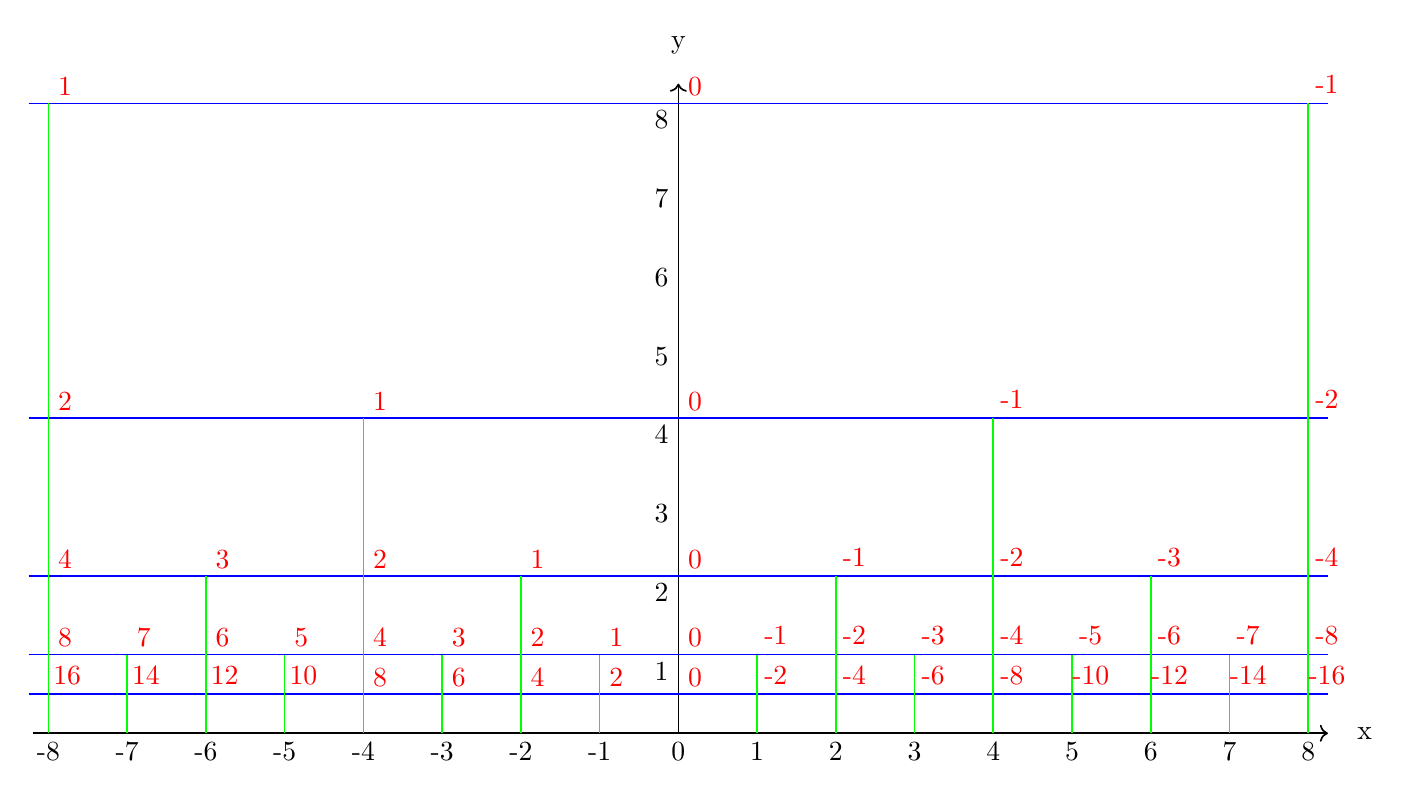
\begin{tikzpicture}
\draw [black, line width=0.6pt, ->] (0,0) to[out=90,in=270] (0,8.25);
\node [anchor=south] at (0,8.5) {y};
\draw [black, line width=0.6pt, ->] (-8.2,0) to[out=0,in=180] (8.25,0);
\node [anchor=west] at (8.5,0) {x};
\foreach \x in {-8,-7,-6,-5,-4,-3,-2,-1,0,1,2,3,4,5,6,7,8}
  \node [anchor=north] at (\x,0) {\x};
\foreach \y in {1,2,3,4,5,6,7,8}
  \node [anchor=45] at (0,\y) {\y};

\draw [blue, line width=0.6pt] (-8.25,0.5) to[out=0,in=180] (8.25,0.5);
\draw [blue, line width=0.6pt] (-8.25,1) to[out=0,in=180] (8.25,1);
\draw [blue, line width=0.6pt] (-8.25,2) to[out=0,in=180] (8.25,2);
\draw [blue, line width=0.6pt] (-8.25,4) to[out=0,in=180] (8.25,4);
\draw [blue, line width=0.6pt] (-8.25,8) to[out=0,in=180] (8.25,8);

\draw [green, line width=0.6pt] (-8,0) to[out=90,in=270] (-8,1);
\draw [green, line width=0.6pt] (-7,0) to[out=90,in=270] (-7,1);
\draw [green, line width=0.6pt] (-6,0) to[out=90,in=270] (-6,1);
\draw [green, line width=0.6pt] (-5,0) to[out=90,in=270] (-5,1);
\draw [green, line width=0.6pt] (-4,0) to[out=90,in=270] (-4,1);
\draw [green, line width=0.6pt] (-3,0) to[out=90,in=270] (-3,1);
\draw [green, line width=0.6pt] (-2,0) to[out=90,in=270] (-2,1);
\draw [green, line width=0.6pt] (-1,0) to[out=90,in=270] (-1,1);
\draw [green, line width=0.6pt] (1,0) to[out=90,in=270] (1,1);
\draw [green, line width=0.6pt] (2,0) to[out=90,in=270] (2,1);
\draw [green, line width=0.6pt] (3,0) to[out=90,in=270] (3,1);
\draw [green, line width=0.6pt] (4,0) to[out=90,in=270] (4,1);
\draw [green, line width=0.6pt] (5,0) to[out=90,in=270] (5,1);
\draw [green, line width=0.6pt] (6,0) to[out=90,in=270] (6,1);
\draw [green, line width=0.6pt] (7,0) to[out=90,in=270] (7,1);
\draw [green, line width=0.6pt] (8,0) to[out=90,in=270] (8,1);

\draw [green, line width=0.6pt] (-8,1) to[out=90,in=270] (-8,2);
\draw [green, line width=0.6pt] (-6,1) to[out=90,in=270] (-6,2);
\draw [green, line width=0.6pt] (-4,1) to[out=90,in=270] (-4,2);
\draw [green, line width=0.6pt] (-2,1) to[out=90,in=270] (-2,2);
\draw [green, line width=0.6pt] (2,1) to[out=90,in=270] (2,2);
\draw [green, line width=0.6pt] (4,1) to[out=90,in=270] (4,2);
\draw [green, line width=0.6pt] (6,1) to[out=90,in=270] (6,2);
\draw [green, line width=0.6pt] (8,1) to[out=90,in=270] (8,2);

\draw [green, line width=0.6pt] (-8,2) to[out=90,in=270] (-8,4);
\draw [green, line width=0.6pt] (-4,2) to[out=90,in=270] (-4,4);
\draw [green, line width=0.6pt] (4,2) to[out=90,in=270] (4,4);
\draw [green, line width=0.6pt] (8,2) to[out=90,in=270] (8,4);

\draw [green, line width=0.6pt] (-8,4) to[out=90,in=270] (-8,8);
\draw [green, line width=0.6pt] (8,4) to[out=90,in=270] (8,8);

\node [anchor=225, red] at (-8,0.5) {16};
\node [anchor=225, red] at (-7,0.5) {14};
\node [anchor=225, red] at (-6,0.5) {12};
\node [anchor=225, red] at (-5,0.5) {10};
\node [anchor=225, red] at (-4,0.5) {8};
\node [anchor=225, red] at (-3,0.5) {6};
\node [anchor=225, red] at (-2,0.5) {4};
\node [anchor=225, red] at (-1,0.5) {2};
\node [anchor=225, red] at (0,0.5) {0};
\node [anchor=225, red] at (1,0.5) {-2};
\node [anchor=225, red] at (2,0.5) {-4};
\node [anchor=225, red] at (3,0.5) {-6};
\node [anchor=225, red] at (4,0.5) {-8};
\node [anchor=225, red] at (5,0.5) {-10};
\node [anchor=225, red] at (6,0.5) {-12};
\node [anchor=225, red] at (7,0.5) {-14};
\node [anchor=225, red] at (8,0.5) {-16};

\node [anchor=225, red] at (-8,1) {8};
\node [anchor=225, red] at (-7,1) {7};
\node [anchor=225, red] at (-6,1) {6};
\node [anchor=225, red] at (-5,1) {5};
\node [anchor=225, red] at (-4,1) {4};
\node [anchor=225, red] at (-3,1) {3};
\node [anchor=225, red] at (-2,1) {2};
\node [anchor=225, red] at (-1,1) {1};
\node [anchor=225, red] at (0,1) {0};
\node [anchor=225, red] at (1,1) {-1};
\node [anchor=225, red] at (2,1) {-2};
\node [anchor=225, red] at (3,1) {-3};
\node [anchor=225, red] at (4,1) {-4};
\node [anchor=225, red] at (5,1) {-5};
\node [anchor=225, red] at (6,1) {-6};
\node [anchor=225, red] at (7,1) {-7};
\node [anchor=225, red] at (8,1) {-8};

\node [anchor=225, red] at (-8,2) {4};
\node [anchor=225, red] at (-6,2) {3};
\node [anchor=225, red] at (-4,2) {2};
\node [anchor=225, red] at (-2,2) {1};
\node [anchor=225, red] at (0,2) {0};
\node [anchor=225, red] at (2,2) {-1};
\node [anchor=225, red] at (4,2) {-2};
\node [anchor=225, red] at (6,2) {-3};
\node [anchor=225, red] at (8,2) {-4};

\node [anchor=225, red] at (-8,4) {2};
\node [anchor=225, red] at (-4,4) {1};
\node [anchor=225, red] at (0,4) {0};
\node [anchor=225, red] at (4,4) {-1};
\node [anchor=225, red] at (8,4) {-2};

\node [anchor=225, red] at (-8,8) {1};
\node [anchor=225, red] at (0,8) {0};
\node [anchor=225, red] at (8,8) {-1};

\end{tikzpicture}
\end{document}
}
    \caption{Conceptual example of a path in the (U,V) reference space. The specific path and values are illustrative and would be adapted based on actual relators from $G(4_1)$.}
    \label{fig:uv_path}
\end{figure}

For example, the net displacement in $U$ or $V$, the enclosed area (if the path forms a closed loop in this space), or the winding number around certain points could be relevant. Figure \ref{fig:uv_path} shows a conceptual representation of such a path. The paths from `knots/results.tex` could be plotted in this space to observe their geometric characteristics.

\subsection{Focus on K=0}
A particular focus will be on identifying conditions that lead to $K=0$. The `knots/results.tex` file notes cases where $p(a)=q(a)$, which corresponds to $K=0$ if the mapping is $S \mapsto (p(a), q(a))$ and torsion is $p(a)-q(a)$. This is significant because it implies $\mathcal{T}(S) = 0$ (assuming $\Delta(t) \neq 0$), which can have profound implications for the arithmetic expression geometry, potentially indicating triviality or a special symmetry of the path under the AEG framework.

\section{Expected Outcomes}
The systematic study is expected to yield:
\begin{itemize}
    \item A deeper understanding of the factors influencing the integer $K$ in the arithmetic torsion formula for the $4_1$ knot, leveraging existing data and new computations.
    \item Heuristic rules or predictive models for $K$ based on path properties (both algebraic and geometric), potentially reducing the need for exhaustive computation for new paths.
    \item Insights into the conditions under which $K=0$, which may highlight special classes of paths or symmetries within the AEG framework for $G(4_1)$, informed by the examples in `knots/results.tex`.
\end{itemize}

This research direction aims to bridge the algebraic definition of arithmetic torsion with the combinatorial and geometric properties of paths in the knot group, providing concrete and valuable insights into the structure of AEG for the $4_1$ knot.

\end{document}

